\documentclass[11pt]{scrartcl}
\usepackage[sexy]{../../../evan}
\usepackage{graphicx}
\usepackage{bm}
\usepackage{pgfplots}
\usetikzlibrary{calc}
\definecolor{dg}{RGB}{2,101,15}
\newtheoremstyle{dotlessP}{}{}{}{}{\color{dg}\bfseries}{}{ }{}
\theoremstyle{dotlessP}
\newtheorem{property}[theorem]{Property}

\newtheoremstyle{dotlessN}{}{}{}{}{\color{teal}\bfseries}{}{ }{}
\theoremstyle{dotlessN}
\newtheorem{notation}[theorem]{Notation}
% Shortcuts
\DeclarePairedDelimiter\ceil{\lceil}{\rceil} % ceil function

\DeclarePairedDelimiter\paren{(}{)} % parenthesis

\newcommand{\df}{\displaystyle\frac} % displaystyle fraction
\newcommand{\qeq}{\overset{?}{=}} % questionable equality

\newcommand{\Mod}[1]{\;\mathrm{mod}\; #1} % modulo operator

\newcommand{\comp}{\circ} % composition

\newcommand{\lra}{\leftrightarrow}

% Text Modifiers
\newcommand{\tbf}{\textbf}
\newcommand{\tit}{\textit}

% Sets
\DeclarePairedDelimiter\set{\{}{\}}
\newcommand{\unite}{\cup}
\newcommand{\inter}{\cap}

\newcommand{\reals}{\mathbb{R}} % real numbers: textbook is Z^+ and 0
\newcommand{\ints}{\mathbb{Z}}
\newcommand{\nats}{\mathbb{N}}
\newcommand{\complex}{\mathbb{C}}
\newcommand{\tots}{\mathbb{Q}}
\newcommand{\smin}{\setminus}
\newcommand{\degree}{^\circ}

% Counting
\newcommand\perm[2][^n]{\prescript{#1\mkern-2.5mu}{}P_{#2}}
\newcommand\comb[2][^n]{\prescript{#1\mkern-0.5mu}{}C_{#2}}

% Relations
\newcommand{\rel}{\mathcal{R}} % relation

\setlength\parindent{0pt}

% Directed Graphs
\usetikzlibrary{arrows}
\tikzset{vertex/.style = {shape=circle,draw,minimum size=2em}}
\tikzset{svertex/.style = {shape=circle,draw,minimum size=.05em,font=\tiny}}
\tikzset{edge/.style = {->,> = latex'}}
\tikzset{dedge/.style = {-> = latex'}}
\tikzset{dot/.style={inner sep=1.5pt,circle,draw,fill}}

% Contradiction
\newcommand{\contradiction}{{\hbox{%
    \setbox0=\hbox{$\mkern-3mu\times\mkern-3mu$}%
    \setbox1=\hbox to0pt{\hss$\times$\hss}%
    \copy0\raisebox{0.5\wd0}{\copy1}\raisebox{-0.5\wd0}{\box1}\box0
}}}
\newcommand{\xxhash}[2]{\rotatebox[origin=c]{#2}{$#1\parallel$}}

\title{MATH 22A: Vector Calculus and Linear Algebra}
\subtitle{PSet 1}
\author{Denny Cao}
\date{\today}
%++++++++++++++++++++++++++++++++++++++++
% Heading and Footer
%++++++++++++++++++++++++++++++++++++++++
% title stuff
\makeatletter
\renewcommand*\env@matrix[1][*\c@MaxMatrixCols r]{%
  \hskip -\arraycolsep
  \let\@ifnextchar\new@ifnextchar
  \array{#1}}
\makeatother

\renewcommand{\maketitle}{\bgroup\setlength{\parindent}{0pt}
	\begin{flushleft}
		\large\textbf{MATH 22A: Vector Calculus and Linear Algebra} \\ \vskip 0.2cm
		\begingroup
		\fontsize{14pt}{12pt}\selectfont
		\title
		\\
		Problem Set 4
		\endgroup \vskip 0.3cm
		Due: Wednesday, October 4, 2023 12pm \hfill\rlap{}\textbf{Denny Cao} \\ \vskip 0.1cm 
		\hrulefill
	\end{flushleft}\egroup
}

\begin{document}
\maketitle
\pagestyle{plain}
\section*{Collaborators}
\begin{itemize}
	\item May Ng
\end{itemize}
\section{Computational Problems}
% Question 1.1
\begin{ques}
	Define the linear transformation $T$ using the matrix below so that $T(x) = Ax$. Find a vector $x$ whose image under $T$ is the vector $b$ depicted below. Also, determine if $x$ is unique.
    \begin{align*}
        A = \begin{bmatrix} 1 & -3 & 2 \\ 0 & 1 & -4 \\ 3 & -5 & -9 \end{bmatrix}, &b = \begin{bmatrix}
            6 \\ -7 \\ -9
        \end{bmatrix}
    \end{align*}
\end{ques}
\textbf{Solution}

We can find $x$ by row reducing the augmented matrix:
\begin{gather*}
	\begin{bmatrix}[rrr|r]
		1 & -3 & 2 & 6 \\
		0 & 1 & -4 & -7 \\
		3 & -5 & -9 & -9
	\end{bmatrix}
	\intertext{$\sim R_3 - 3R_1 \to R_3$.}
	\begin{bmatrix}[rrr|r]
		1 & -3 & 2 & 6 \\
		0 & 1 & -4 & -7 \\
		0 & 4 & -15 & -27 
	\end{bmatrix}
	\intertext{$\sim R_1 + 3R_2 \to R_1$ and $R_3 - 4R_2 \to R_3$.}
	\begin{bmatrix}[rrr|r]
		1 & 0 & -10 & -15 \\
		0 & 1 & -4 & -7 \\
		0 & 0 & 1 & 1
	\end{bmatrix}
	\intertext{$\sim R_1 + 10R_3 \to R_1$ and $R_2 + 4R_3 \to R_2$.}
	\begin{bmatrix}[rrr|r]
		1 & 0 & 0 & -5 \\
		0 & 1 & 0 & -3 \\
		0 & 0 & 1 & 1
	\end{bmatrix}
\end{gather*}
\textbf{Thus, the vector $x$ whose image under $T$ is $b$ is $x = \begin{bmatrix}
		-5 \\
		-3 \\
		1
	\end{bmatrix}$
.}
\\

\textbf{$x$ is unique as any $x$ whose image is $b$ must satisfy $Ax = b$. From Theorem 2 (Uniqueness and Existence Theorem) in Linear Algebra and Its Applications, as the rightmost column of the reduced augmented matrix is not a pivot column, the system is consistent. As the system is consistent and has no free variables, then the solution set contains a unique solution. Thus, $x$ is unique.}

% Question 1.2
\begin{ques}
	Define the matrix $A$ and vector $b$ as done below. Is $b$ in the range of the linear transformation $T(x) = Ax$? If so, find $x$; if not then why not?
    \begin{align*}
        A = \begin{bmatrix}
            1 & 3 & 9 & 2 \\ 1 & 0 & 3 & -4 \\ 0 & 1 & 2 & 3 \\ -2 & 3 & 0 & 5
        \end{bmatrix}, &b = \begin{bmatrix}
            -1 \\ 3 \\ -1 \\ 4
        \end{bmatrix}
    \end{align*}
\end{ques}
\textbf{Solution}

If $b$ is in the range of the linear transformation $T(x) = Ax$, then $b$ is a linear combination of the columns of $A$; there will exist a solution to the augmented matrix below:
\begin{gather*}
	\begin{bmatrix}[rrrr|r]
	1 & 3 & 9 & 2 & -1 \\
	1 & 0 & 3 & -4 & 3 \\
	0 & 1 & 2 & 3 & -1 \\
	-2 & 3 & 0 & 5 & 4
	\end{bmatrix}
	\intertext{$\sim R_2 - R_1 \to R_2$ and $R_4 + 2R_1 \to R_4$.}
	\begin{bmatrix}[rrrr|r]
	1 & 3 & 9 & 2 & -1 \\
	0 & -3 & -6 & -6 & 4 \\
	0 & 1 & 2 & 3 & -1 \\
	0 & 9 & 18 & 9 & 2
	\end{bmatrix}
	\intertext{$\sim R_2 + 3R_3 \to R_3$ and $3R_2 + R_4 \to R_4$.}
	\begin{bmatrix}[rrrr|r]
	1 & 3 & 9 & 2 & -1 \\
	0 & -3 & -6 & -6 & 4 \\
	0 & 0 & 0 & 3 & 1 \\
	0 & 0 & 0 & -9 & 14 
	\end{bmatrix}
	\intertext{$\sim 3R_3 + R_4 \to R_4$.}
	\begin{bmatrix}[rrrr|r]
	1 & 3 & 9 & 2 & -1 \\
	0 & -3 & -6 & -6 & 4 \\
	0 & 0 & 0 & 3 & 1 \\
	0 & 0 & 0 & 0 & 17
	\end{bmatrix}
\end{gather*}
As we reach an augmented matrix in an echelon form and the rightmost column is a pivot column, by Theorem 2 (Existence and Uniqueness Theorem) in Linear Algebra and Its Applications, the system is not consistent and thus there does not exist a solution.
\\

Thus, $b$ is not a linear combination of the columns of $A$ and thus is not in the range of the linear transformation $T(x) = Ax$.
% Question 1.3
\begin{ques}
	Let $u$ and $v$ be linearly independent vectors in $\mathbb{R}^3$ and let $P$ denote the plane containing these vectors and $0$. The parametric equation for P is $x = tu+sv$ for $s,t \in \mathbb{R}$. Let $w$ denote a vector in $\mathbb{R}^3$ that is such that every vector in $\mathbb{R}^3$ can be written as $c_1u+c_2v+c_3w$ for some choice of numbers $c_1,c_2$ and $c_3$ (Any vector that points out of P is sufficient for this purpose). In terms of $u,v$ and $w$ give a linear transformation $T: \mathbb{R}^3 \to \mathbb{R}^3$ that maps P onto a plane, then give one that maps P onto a line, and then give one (not identically 0) that maps all of P to the origin. What must be true of $T(u)$ and $T(v)$ for the image of P to be a plane?
\end{ques}
\textbf{Solution}

The linear transformation $T$ maps $P$ to the parametric equation:
\begin{align*}
	T(x) &= T(t\vec{u} = s\vec{v}) \\
		 &= tT(\vec{u}) + sT(\vec{v})
\end{align*}
The linear transformation will map $P$ to a plane if $T(\vec{u}) \neq \vec{0}$ and $T(\vec{v}) \neq \vec{0}$ and $T(\vec{u})$ and $T(\vec{v})$ must be linearly independent. This is because, if they are linearly independent, $P$ will $\text{Span}(T(\vec{u}), T(\vec{v}))$, and if they are not linearly independent, then either $T(\vec{u})$ or $T(\vec{v})$ can be expressed as a linear combination of the other, which would reduce $T(x)$ to a line. For instance, let $T(\vec{u}) = bT(\vec{v})$. Then, $T(x) = \displaystyle\frac{t}{b}T(\vec{v}) + sT(\vec{v}) = \displaystyle\frac{t + sb}{b}T(\vec{v})$.
\\

The linear transformation will map $P$ to a line if  $T(\vec{u}) = \vec{0}$ or $T(\vec{v}) = \vec{0}$, but not both, as then $T(x) = tT(\vec{u})$ or $T(x) = sT(\vec{v})$. It will also be a line in the case above, where $T(\vec{u})$ and $T(\vec{v})$ are linearly dependent.
\\

A linear transformation that would map $P$ to the origin would be a linear transformation where $T(\vec{u}) = \vec{0}, T(\vec{v}) = \vec{0}, T(\vec{w}) = \vec{w}$, as $T(x) = tT(\vec{u}) + sT(\vec{v}) = t(\vec{0}) + s(\vec{0}) = \vec{0}$.
\\


% Question 1.4
\begin{ques}
	An \emph{affine} transformation $T: \mathbb{R}^n \to \mathbb{R}^m$ has the form $T(x) = Ax+b$ with $A \in \mathbb{R}^{m \times n}$ (A is an $m \times n$ matrix) and with $b$ being a vector in $\mathbb{R}^m$. Explain why $T$ is not linear except if $b = 0$. 
\end{ques}
\textbf{Solution}

If $T$ is linear, then $T(\bm{0}) = \bm{0}$. As $T(\bm{x}) = A\bm{x} + \bm{b}$, $T(\bm{0}) = A(\bm{0}) + \bm{b} = \bm{b}$. $T(\bm{0}) = \bm{0}$ is only true when $\bm{b} = \bm{0}$.
% Question 1.5
\begin{ques}
	Let $T: \mathbb{R}^3 \to \mathbb{R}^3$
denote the transformation that projects each vector $x$ onto the $x_2 = 0$ plane. Show that $T$ is a linear transformation and write its standard matrix.
\end{ques}
\textbf{Solution}

A transformation is linear if:
\begin{enumerate}[i.]
	\item $\forall u, v \in \reals^3(T(\bm{u} + \bm{v}) = T(\bm{u}) + T(\bm{v}))$ 
	\item $\forall u \in \reals, v \in \reals^3(T(c\bm{u}) = cT(\bm{u}))$
\end{enumerate}
Let $\bm{u} = 
\begin{bmatrix}
	u_1 \\
	u_2 \\
	u_3
\end{bmatrix}
$ and $\bm{v} = 
\begin{bmatrix}
	v_1 \\
	v_2 \\
	v_3
\end{bmatrix}
$. Then, $T(\bm{u}) = 
\begin{bmatrix}[c]
	u_1 \\
	0 \\
	u_3
\end{bmatrix}
$ and $T(\bm{v}) = 
\begin{bmatrix}[c]
	v_1 \\
	0 \\
	v_3
\end{bmatrix}
$. Thus: 
\[
T(\bm{u}) + T(\bm{v}) = \begin{bmatrix}[c]
	u_1 \\
	0 \\
	u_3
\end{bmatrix} +
\begin{bmatrix}[c]
	v_1 \\
	0 \\
	v_3
\end{bmatrix} =
\begin{bmatrix}[c]
	u_1 + v_1 \\
	0 \\
	u_3 + v_3
\end{bmatrix}
\] 
As $\bm{u} + \bm{v} = 
\begin{bmatrix}
	u_1 \\
	u_2 \\
	u_3
\end{bmatrix} +
\begin{bmatrix}
	v_1 \\
	v_2 \\
	v_3
\end{bmatrix} = 
\begin{bmatrix}
	u_1 + v_1 \\
	u_2 + v_2 \\
	u_3 + v_3
\end{bmatrix} 
$:
\[
	T(\bm{u} + \bm{v}) = 
	\begin{bmatrix}[c]
		u_1 + v_1 \\
		0 \\
		u_3 + v_3
	\end{bmatrix}
\]
Thus, the first property is met.
\\

For the second case, $c\bm{u} = c 
\begin{bmatrix}
	u_1 \\
	u_2 \\
	u_3
\end{bmatrix} = 
\begin{bmatrix}
	c u_1 \\
	c u_2 \\
	c u_3
\end{bmatrix}
$. Thus:
\[
	T(c\bm{u}) = 
	\begin{bmatrix}[c]
		cu_1 \\
		0 \\
		cu_3
	\end{bmatrix}
\] 
As $T(\bm{u}) = 
\begin{bmatrix}[c]
	u_1 \\
	0 \\
	u_3
\end{bmatrix}
$:
\[
	cT(\bm{u}) = c\begin{bmatrix}[c]
	u_1 \\
	0 \\
	u_3
\end{bmatrix} = 
\begin{bmatrix}[c]
	cu_1 \\
	0 \\
	cu_3
\end{bmatrix}
\]
Thus, the second property is met. As both properties are met, the transformation is linear.
\\

The standard matrix of $T$ is:
\[
A = \begin{bmatrix}
	1 & 0 & 0 \\
	0 & 0 & 0 \\
	0 & 0 & 1
\end{bmatrix}
\] 
% Question 1.6
\begin{ques}
Find the standard matrix for the linear transformation $T: \mathbb{R}^3 \to \mathbb{R}^2$ if $T$ maps the columns $e_1$, $e_2$, $e_3$ of the $3 \times 3$ identity matrix as depicted below.
\begin{center}
    $T(e_1) = \begin{bmatrix}
        -5 \\ 4
    \end{bmatrix}, T(e_2) = \begin{bmatrix}
        4 \\ -7
    \end{bmatrix}, T(e_3) = \begin{bmatrix}
        1 \\ 3
    \end{bmatrix}$
\end{center}
\end{ques}
\textbf{Solution}

The standard matrix is:
\[
A = \begin{bmatrix}
	-5 & 4 & 1 \\
	4 & -7 & 3
\end{bmatrix}
\] 
% Question 1.7
\begin{ques}
	Let $T: \mathbb{R}^2 \to \mathbb{R}^2$ be a linear transformation with standard matrix $A = [a_1, a_2]$ where $a_1$ and $a_2$ are as depicted in the figure below. Using the figure, draw the image of $\begin{bmatrix}
    -1 \\ 3
\end{bmatrix}$ by $T$.

\begin{center}
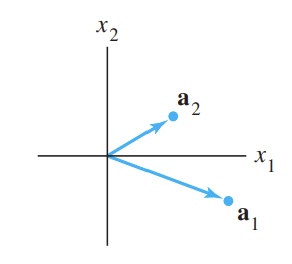
\includegraphics[]{screen2.png}
\end{center}
\end{ques}
\textbf{Solution}	
\begin{center}
\begin{tikzpicture}
\begin{axis}[
  axis lines=middle,
  xlabel=$x$, xlabel style={at=(current axis.right of origin), anchor=west},
  ylabel=$y$, ylabel style={at=(current axis.above origin), anchor=south},
  axis line style={-,thick},
  scale only axis,
  xmin=-3,xmax=4,ymin=-1.5,ymax=4,
  xlabel=$x_1$,
  ylabel=$x_2$,
  ticks=none]
% Define the coordinates of the unit vector with angle 30 degrees
\newcommand{\thetao}{30}
\newcommand{\thetat}{-20}
\newcommand{\s}{3}
\newcommand{\m}{1.5}
\coordinate (O) at (axis cs:0,0); % Origin
\coordinate (A) at (axis cs:{\m*cos(\thetao)},{\m*sin(\thetao)}); % Endpoint of the unit vector
\coordinate (B) at (axis cs:{\s*cos(\thetat}, {\s*sin(\thetat});
\coordinate (C) at (axis cs:{\s*cos(-180 + \thetat)}, {\s*sin(-180 + \thetat)});
\node[circle, draw, fill=blue, inner sep=2pt, label=$a_2$]  at (A) {};
\node[circle, draw, fill=blue, inner sep=2pt, label=$a_1$]  at (B) {};
\coordinate (D) at (axis cs:{3*\m*cos(\thetao)},{3*\m*sin(\thetao)}); % Endpoint of the unit vector
\coordinate (E) at (axis cs:{3*\m*cos(\thetao) + \s*cos(180 - \thetao)},{3*\m*sin(\thetao) + \s*sin(180 - \thetao)});% Draw the unit vector

\draw[-stealth,cyan,thick] (O) -- (A);
\draw[-stealth,cyan,thick] (O) -- (B);
\draw[-stealth, dashed, black,thin] (O) -- (C);
\draw[-stealth, dashed, black,thin] (A) -- (D);
\draw[-stealth, dashed, black,thin] (C) -- (E);
\draw[-stealth, dashed, black,thin] (D) -- (E);
\draw[-stealth,red,very thick] (O) -- (E);
\end{axis}
\end{tikzpicture}
\end{center}
% Question 1.8
\begin{ques}
	Give the matrix that implements the transformation $T: \mathbb{R}^2 \to \mathbb{R}^4$ that is given by the rule whereby $T(x_1\vec{e_1} + x_2\vec{e_2})$ is sent to 
\[
	\begin{bmatrix}[c]
        2x_2-3x_1 \\ x_1-4x_2 \\ 0 \\ x_2
    \end{bmatrix}
\] 
\end{ques}
\textbf{Solution}

We determine the matrix that implements the transformation $T$ by analyzing what happens to the basis vectors:
 \begin{align*}
	 T\paren*{\vec{i}
	 } = 
	 \begin{bmatrix}
	 	-3 \\
		1 \\
		0 \\
		0
	 \end{bmatrix} \quad
	 T
	 \paren*{\vec{j}
	 } =
	 \begin{bmatrix}
	 	2 \\
		-4 \\
		0 \\
		1
	 \end{bmatrix}
\end{align*}
Thus, the matrix that implements the transformation $T$ is:
\[
\begin{bmatrix}
	-3 & 2 \\
	1 & -4 \\
	0 & 0 \\
	0 & 1
\end{bmatrix}
\] 
% Question 1.9
\begin{ques}
	Let $T$ be the linear transformation whose standard matrix is given below. Is $T$ a 1-1 mapping? Is is an onto mapping? Justify your answers. 
\begin{align*}
    &\begin{bmatrix}
        7 & 5 & 4 & -9 \\ 10 & 6 & 16 & -4 \\ 12 & 8 & 12 & 7 \\ -8 & -6 & -2 & 5
    \end{bmatrix} 
\end{align*}
\end{ques}
\textbf{Solution}

By Theorem 11 in Linear Algebra and Its Applications, $T$ is a one-to-one function if and only if $T(\vec{x}) = \vec{0}$ has only the trivial solution. We reduce the augmented matrix:
\begin{gather*}
	\begin{bmatrix}[rrrr|r]
		7 & 5 & 4 & -9 & 0 \\
		10 & 6 & 16 & -4 & 0 \\
		12 & 8 & 12 & 7 & 0 \\
		-8 & -6 & -2 & 5 & 0 
	\end{bmatrix}
	\intertext{$\sim R_4 + R_1 \to R_4$.}
	\begin{bmatrix}[rrrr|r]
		7 & 5 & 4 & -9 & 0 \\
		10 & 6 & 16 & -4 & 0 \\
		12 & 8 & 12 & 7 & 0 \\
		-1 & -1 & 2 & -4 & 0 
	\end{bmatrix}
	\intertext{$\sim -R_4 \leftrightarrow R_1$.}
	\begin{bmatrix}[rrrr|r]
		1 & 1 & -2 & 4 & 0 \\
		10 & 6 & 16 & -4 & 0 \\
		12 & 8 & 12 & 7 & 0 \\
		7 & 5 & 4 & -9 & 0
	\end{bmatrix}
	\intertext{$R_2 - 10R_1 \to R_2, R_3 - 12R_1 \to R_3, $ and $R_4 - 7R_1 \to R_4$.}
	\begin{bmatrix}[rrrr|r]
		1 & 1 & -2 & 4 & 0 \\
		0 & -4 & 36 & -44 & 0 \\
		0 & -4 & 36 & -41 & 0 \\
		0 & -2 & 18 & -37 & 0
	\end{bmatrix}
	\intertext{$R_2 - 10R_1 \to R_2, R_3 - 12R_1 \to R_3, $ and $R_4 - 7R_1 \to R_4$.}
	\begin{bmatrix}[rrrr|r]
		1 & 1 & -2 & 4 & 0 \\
		0 & -4 & 36 & -44 & 0 \\
		0 & -4 & 36 & -41 & 0 \\
		0 & -2 & 18 & -37 & 0
	\end{bmatrix}
	\intertext{$\sim R_3 - R_2 \to R_3$ and $2R_4 - R_2 \to R_4$.}
	\begin{bmatrix}[rrrr|r]
		1 & 1 & -2 & 4 & 0 \\
		0 & -4 & 36 & -44 & 0 \\
		0 & 0 & 0 & 3 & 0 \\
		0 & 0 & 0 & -30 & 0
	\end{bmatrix}
	\intertext{$\sim R_4 + 10R_3 \to R_4$.}
	\begin{bmatrix}[rrrr|r]
		1 & 1 & -2 & 4 & 0 \\
		0 & -4 & 36 & -44 & 0 \\
		0 & 0 & 0 & 3 & 0 \\
		0 & 0 & 0 & 0 & 0
	\end{bmatrix}
\end{gather*}
We reach an augmented matrix in echelon form and can observe that there exists a free variable. Thus, there are infinitely many solutions to the system, meaning $T$ is not one-to-one.
\\

$T$ is not onto. By Theorem 12, $T$ maps $\reals^n$ onto $\reals^m$ if and only if the columns of $A$ span $\reals^m$. By Theorem 4, as $A$ does not have a pivot position in every row, the columns of $A$ do not span $\reals^m$.
% Question 1.10
\begin{ques}
	Find numbers $a,b$ such that the following holds: 
\begin{align*}
    \begin{bmatrix}
        a & 0 & -b \\ 0 & 1 & 0 \\ b & 0 & a
    \end{bmatrix} \begin{bmatrix}
        2 \\ 3 \\ 4
    \end{bmatrix} &= \begin{bmatrix}
        2\sqrt{5} \\ 3 \\ 0
    \end{bmatrix}, a^2+b^2=1 
\end{align*}
\end{ques}
\textbf{Solution}

We set up a system:
\begin{align*}
	2a - 4b &= 2\sqrt{5} \\
	3 &= 3 \\
	2b + 4a &= 0
\end{align*}
Thus:
\begin{align*}
	a - 2b &= \sqrt{5} \\
	b + 2a &= 0 
\end{align*}
From the second equation, $b = -2a$. We substitute into the first equation:
\begin{align*}
	a - 2(-2a) &= \sqrt{5} \\
	5a &= \sqrt{5} \\
	a &= \frac{\sqrt{5}}{5}
\intertext{We substitute into $b = -2a$:}
	b &= -2\paren*{\frac{\sqrt{5}}{5}}
\end{align*}
We check that this satisfies $a^2 + b^2 = 1$:
\begin{align*}
	\paren*{\frac{\sqrt{5}}{5}}^2 + \paren*{\frac{-2\sqrt{5}}{5}}^2 &= \frac{5}{25} + \frac{4(5)}{25} \\
																	&= \frac{1}{5} + \frac{4}{5} \\
																	&= 1
\end{align*}
Thus, the numbers $a,b$ are:
\begin{align*}
	a = \frac{\sqrt{5}}{5}\quad b = \frac{-2\sqrt{5}}{5}
\end{align*}
\section{Proof Problems}
% Question 2.1
\begin{ques}
An interesting function. Let $\mathbb{Z}^+$ be the set of positive integers. Consider the function $g: \mathbb{Z} \to \mathbb{Z}^+$ given by
    \begin{align*}
        g(k) &= \begin{cases}
            2k+1 & \text{if $k \geq 0$} \\
            -2k & \text{if $k<0$}
        \end{cases}
    \end{align*}
    \begin{itemize}
        \item[(a)] Show that $g$ is a surjecive function.
        \item[(b)] Show that $g$ is an injective function.
        \item[(c)] Conclude that $g$ is a bijective function.
    \end{itemize}
\end{ques}
\textbf{Solution}

\begin{enumerate}[(a)]
	\item  \
	\begin{claim*}
		$g$ is surjective.
	\end{claim*}
	\begin{proof}
		We will show that, for all $y \in \ints^+$, there exists a $x \in \ints$ such that $g(x) = y$.
		\\

The set of positive integers $\ints^+$ can be divided into two subsets: the positive even numbers and the positive odd numbers. Thus, to establish the surjectiveness of $g$, it is enough to demonstrate that for any positive even number $y_1$ and any positive odd number $y_2$, there exist integers $x_1$ and $x_2$ in the domain of $g$ such that $g(x_1) = y$ and $g(x_2) = z$, respectively.
\\

		Without loss of generality, let $y_1$ be a positive odd number. By definition of odd number, $y_1 = 2c + 1, c \in \nats$. Let  $x_1 = c$. Then, $x_1 = c \geq 0$, satisfying the first condition of the piecewise function. Thus, $g(x_1) = g(c) = 2c+1 = y_1$. We have shown that, for all positive odd numbers  $y_1$, there exists a $x \in \nats$, and as $\nats \subset \ints$, a $x_1 \in \ints$ (the domain of $g$) such that $g(x_1)=y_1$.
\\

		Without loss of generality, let $y_2$ be a positive even number. By definition of positive even number, $y_2 = 2c, c \in \ints^+$. Let  $x_2 = -c$. Then, $x_2 = -c < 0$, satisfying the second condition of the piecewise function. Thus, $g(x_2) = g(-c) = -2(-c) = 2c = y_2$. We have shown that, for all positive even numbers $y_2$, there exists a  $x_2 \in \ints$ (the domain of $g$) such that $g(x_2) = y$.
		\\

As for all positive odd numbers $y_1$ and all positive even numbers $y_2$, there exist integers $x_1$ and $x_2$ such that $g(x_1) = y_1$ and $g(x_2) = y_2$, we can conclude that $g$ is surjective, covering the entire range of positive integers $\ints^+$. Therefore, the function $g$ is surjective, and the proof is complete.
	\end{proof}
\item \
	\begin{claim*}
		$g$ is injective.
	\end{claim*}
	\begin{proof}
		[Proof by contrapositive]
		We will show that, for all $x_1, x_2 \in \ints$, $g(x_1) = g(x_2) \implies x_1 = x_2$ by observing the 4 possible cases: $x_1 \geq 0 \land x_2 < 0$, $x_1 < 0 \land x_2 \geq 0$, $x_1 \geq 0 \land x_2 \geq 0$, and $x_1 < 0 \land x_2 < 0$.
		\\

		We verify that, when  $x_1 \geq 0$ and $x_2 < 0$, $g(x_1) \neq g(x_2)$. When  $x_1 \geq 0$, $g(x_1) = 2x_1 + 1$. When $x_2 < 0$, $g(x_2) = -2x_2$.
		\begin{align*}
			2x_1 + 1 &\stackrel{?}{=} -2x_2 \\
			2x_1 + 2x_2 &\stackrel{?}{=} -1 \\
			x_1 + x_2 &\stackrel{?}{=} -\frac{1}{2}
		\end{align*}
		As $x_1, x_2 \in \ints$, $x_1 + x_2 \neq -\displaystyle\frac{1}{2}$, and thus it is never the case that $g(x_1) = g(x_2)$ when $x_1 \geq 0$ and $x_2 < 0$. A symmetrical argument can be made for when $x_1 < 0$ and $x_2 \geq 0$.
		\\

		We will now examine two cases:
		\begin{enumerate}[(i)]
			\item $x_1 \geq 0$ and $x_2 \geq 0$. Then, $g(x_1) = 2x_1 + 1$ and $g(x_2) = 2x_2 + 1$. If $g(x_1) = g(x_2)$, then:
				\begin{align*}
					2x_1 + 1 &= 2x_2 + 1 \\
					2x_1 &= 2x_2 \\
					x_1 &= x_2
		        \end{align*}
			\item $x_1 < 0$ and $x_2 < 0$. Then, $g(x_1) = -2x_1$ and $g(x_2) = -2x_2$. If $g(x_1) = g(x_2)$, then:
				\begin{align*}
					-2x_1 &= -2x_2 \\
					x_1 &= x_2
				\end{align*}
		\end{enumerate}
		As we have shown that for all $x_1, x_2  \in \ints$, if $g(x_1) = g(x_2)$, then $x_1 = x_2$, we can conclude that $g$ is injective and the proof is complete.
		\end{proof}
	\item \
		\begin{claim*}
			$g$ is bijective.
		\end{claim*}
		\begin{proof}
			A function is bijective if and only if it is injective and surjective. From (a) and (b),  $g$ is surjective and injective. Thus, $g$ is bijective.
		\end{proof}
	\end{enumerate}
% Question 2.2
\begin{ques}
	Let $T: \reals^2 \to \mathbb{R}^3$ be a linear transformation and $v_1,v_2,v_3$ be three vectors in the range of T. Prove that these three vectors are linearly dependent.
\end{ques}
\textbf{Solution}
\begin{proof}
	As $\vec{v_1}, \vec{v_2}, \vec{v_3}$ are in the range of $T$, there exists  $\vec{x_1}, \vec{x_2}, \vec{x_3} \in \reals^2$ such that $T(\vec{x_1}) = \vec{v_1}$, $T(\vec{x_2}) = \vec{v_2}$, and $T(\vec{x_3}) = \vec{v_3}$. As the set of vectors $\vec{v_1}, \vec{v_2}, \vec{v_3}$ contains more vectors than there are entries in each vector, by Theorem 8 in Linear Algebra and Its Applications, the set is linearly dependent. Thus, by definition of linear dependence, there exist weights $c_1, c_2, c_3$ not all zero such that
	\[
		c_1 \vec{x_1} + c_2 \vec{x_2} + c_3 \vec{x_3} = \vec{0}
	\] 
	We apply a linear transformation to the equation:
	\begin{align*}
		T(c_1 \vec{x_1} + c_2 \vec{x_2} + c_3 \vec{x_3}) &= T(\vec{0}) \\
		\intertext{We use properties of linear transformations to rewrite the equation:}
		T(c_1 \vec{x_1}) + T(c_2 \vec{x_2}) + T(c_3\vec{x_3}) &= T(\vec{0}) \\
		c_1T(\vec{x_1}) + c_2T(\vec{x_2}) + c_3T(\vec{x_3}) &= \vec{0}
		\intertext{We substitute $\vec{v_1}, \vec{v_2}, \vec{v_3}$ for $T(\vec{x_1}), T(\vec{x_2}), T(\vec{x_3})$ respectively:}
		c_1\vec{v_1} + c_2\vec{v_2} + c_3\vec{v_3} &= \vec{0}
	\end{align*}
	Thus, as there exists weights $c_1,c_2,c_3$ not all zero such that 	$c_1\vec{v_1} + c_2\vec{v_2} + c_3\vec{v_3} = \vec{0}$, $\vec{v_1}, \vec{v_2}, \vec{v_3}$ are linearly dependent.
\end{proof}
% Question 2.3
\begin{ques}
    Prove by mathematical induction (being very careful to explain what you are doing at each step) that for every positive integer $n$ we have: 
    \begin{align*}
        1+8+27+\dots+n^3 &= \left( \dfrac{n(n+1)}{2}\right)^2
    \end{align*}
\end{ques}
\textbf{Solution}

	\begin{claim*}
		For every positive integer $n$:
		\[
			1 + 8 + 27 + \dots + n^3 = \paren*{\frac{n(n+1)}{2}}^2
		\] 
	\end{claim*}
	\begin{proof}
		[Proof by induction]
		Let $P(n)$ be the statement that $1 + 8 + 27 + \dots + n^3  = \displaystyle\paren*{\frac{n(n+1)}{2}}^2$. We will show by induction that, for all $n \in \ints^+$, $P(n)$ is true.
		\\

		\textit{Base Case}: $n = 1$. Then, $1^3 = 1$ and $\displaystyle\paren*{\frac{1(1+1)}{2}}^2 = \displaystyle\paren*{\frac{2}{2}}^2 =  1^2 = 1$. Thus, $P(1)$ is true.
		\\

		\textit{Inductive Hypothesis}: Assume that $P(k)$ is true, $k \in \ints^+$ and $k > 1$. We will show that $P(k) \implies P(k+1)$.
		\\

		\textit{Inductive Step}: As $P(k)$ is true:
		\[
		1 + 8 + 27 + \dots + k^3 = \paren*{\frac{k(k+1)}{2}}^2		
		\] 
		We add $(k+1)^3 $ to both sides:
		\begin{align*}
			1 + 8 + 27 + \dots + k^3 + (k+1)^3 &= \paren*{\frac{k(k+1)}{2}}^2 + (k+1)^3 \\
										   &= \frac{k^2(k+1)^2}{4} + (k+1)^3 \\
										   &= (k+1)^2 \paren*{\frac{k^2}{4} + (k+1)} \\
										   &= (k+1)^2 \paren*{\frac{k^2 + 4k + 4}{4}} \\
										   &= (k+1)^2 \paren*{\frac{(k+2)^2}{2^2}} \\
										   &= \frac{(k+1)^2(k+2)^2}{2^2} \\
			1 + 8 + 27 + \dots + k^3 + (k+1)^3 &= \paren*{\frac{(k+1)(k+2)}{2}}^2
		\end{align*}
		We have shown that $P(k) \implies P(k+1)$. Thus, by induction, $P(n)$ is true for all $n \in \ints^+$ and the proof is complete.
	\end{proof}
% Question 2.4
\begin{ques}
	What's wrong with the following `proof' that all buildings have the same height? \\
\textbf{Claim:} All buildings have the same height. \\
\textbf{Proof by induction}: We will prove the statement by induction on the number of buildings. For the base case (n = 1), when we have only 1 building, that building has the same height as itself, so the base case holds. For the inductive step, our inductive hypothesis is that in any collection of n buildings, all the buildings will have the same height. We need to show that for any collection of n + 1 buildings, we have that all the buildings have the same height. Suppose the heights are given by $h_1,\dots,h_{n+1}$. Applying the inductive hypothesis to the first n buildings, we get the first n buildings have the same height; namely, $h_1 = \dots = h_n$. Applying the inductive hypothesis to the last n buildings, we get $h_2 = \dots = h_{n+1}$. But now the middle buildings, $h_1 = \dots = h_n$ belong to both sets, so they have the same height as $h_1$ and $h_{n+1}$. Thus all n+1 buildings have the same height, and by the principle of mathematical induction, all buildings have the same height.
\end{ques}
\textbf{Solution}

The problem lies in the fact that the intersection of the two collections of buildings is used to prove that $h_1 = h_{n+1}$.  Consider the case when $n+1 = 2$. Then, the only heights are  $h_1$ and $h_2$, meaning one collection would contain only $h_1$ and the other would only contain $h_2$. As there is no building in both collections, $h_1$ and $h_2$ do not necessarily have to be the same. 
% Question 2.5
\begin{ques}
	[Extra Credit] The Fibonacci Squares. The Fibonacci sequence is the sequence $1,1,2,3,5,8,\dots$ given by $f_1 = 1$, $f_2 = 1$ and for any $i \geq 3$, $f_i = f_{i-1} + f_{i_2}$. 
\begin{itemize}
    \item Prove by induction that for any natural number $n$, we get $f_1^2 + f_2^2 + \dots + f_n^2 = f_nf_{n+1}$
    \item Another way to argue that the equality above holds is to examine the picture on the left. You don't need to write anything down for this part of the problem, but do look at the image (ignore the spiral) and try to figure out how this picture is a proof of the equation. 
    \begin{center}
        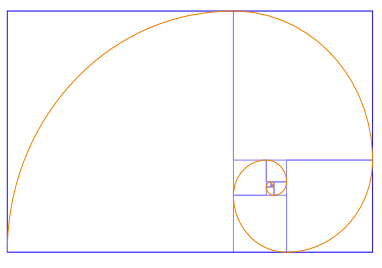
\includegraphics[width=0.5\textwidth]{Immagine 2023-09-29 185814.png}
    \end{center}
\end{itemize}
\end{ques}
\textbf{Solution}
	\begin{claim*}
		For any natural number $n$, $f_1^2 + f_2^2 + \dots + f_n^2 = f_n f_{n+1}$, where $f_1 = 1, f_2 = 1$ and for any $i \geq 3, f_i = f_{i-1} + f_{i-2}$.
	\end{claim*}
\begin{proof}
	[Proof by induction] Let $P(n)$ be the statement that, $f_1^2 + f_2^2 + \dots + f_n^2 = f_n f_{n+1}$. We will show by induction that, for all $n \in \ints^+$, $P(n)$ is true.
	\\

	\textit{Base Case}: $n=1$. $f_1^2 = 1^2 = 1$ and $f_1 f_{2} = 1(1) = 1$. Thus,  $P(1)$ is true.
	\\

	\textit{Inductive Hypothesis}: Assume that $P(k)$ is true, $k \in \ints^+$ and $k > 1$. We will show that $P(k) \implies P(k+1)$.
	\\

	\textit{Inductive Step}: As $P(k)$ is true:
	\[
		f_1^2 + f_2^2 + \dots + f_k^2 = f_k f_{k+1}
	\] 
	We add $f_{k+1}^2$ to both sides:
	\begin{align*}
		f_1^2 + f_2^2 + \dots + f_k^2 + f_{k+1}^2 &= f_k f_{k+1} + f_{k+1}^2 \\
												  &= f_{k+1}(f_k + f_{k+1})
												  \intertext{By definition, $f_i = f_{i-1} + f_{i-2}$. Let  $i = k+2$. Then, $f_{k+2} = f_{k+1} + f_{k}$. Thus:}
		f_1^2 + f_2^2 + \dots + f_k^2 + f_{k+1}^2 &= f_{k+1}(f_{k+2})
	\end{align*}	
	We have shown that $P(k) \implies P(k+1)$. Thus, by induction, $P(n)$ is true for all $n \in \ints^+$ and the proof is complete.
\end{proof}
\section{Science Problem}
\begin{ques}
	What is the matrix $A$ if the correct horizontal and vertical scales are 25 km instead of 30 km?	
\end{ques}
\textbf{Solution}
\[
A =	\begin{bmatrix}
		\frac{5}{6} & 0 \\
		0 & \frac{5}{6}
	\end{bmatrix}
\] 
\begin{ques}
	How do our upper bound of 3900 and our lower bound of 2825 square kilometers change if the correct horizontal and verticale scales are 25 km instead of 30 km?
\end{ques}
\textbf{Solution}

As the upper and lower bounds are obtained by the sum of squares, and the squares are scaled down by a factor of $\displaystyle\frac{5}{6}$ on both sides, the upper and lower bounds will decrease by a factor of  $\paren*{\displaystyle\frac{5}{6}}^2 = \displaystyle\frac{25}{36}$. Thus, the upper bound would become approximately 2708.33 $\text{km}^2$ and the lower bound would become approximately 1961.81 $\text{km}^2$.
\begin{ques}
	What would the matrix $A$ be in this case described above?
\end{ques}
\textbf{Solution}
\[
A = 
\begin{bmatrix}[cc]
	\displaystyle\frac{1}{\cos \frac{\pi}{4}} & 0 \\
	0 & 1 
\end{bmatrix}
\] 
\begin{ques}
	How would the upper and lower bounds of 3900 and 2825 for the area of A--68A change if the foreshortening effect described above were actually present?	
\end{ques}
\textbf{Solution}

As only the $x$ distance is scaled down by a factor of $\cos \displaystyle \frac{\pi}{4}$, the area will be scaled down by the same factor. Thus, the upper bound will be approximately 5515.43 $\text{km}^2$ and the lower bound will be approximately 3995.15 $\text{km}^2$.
\end{document}

